% !TEX root = paper.tex

% Programming multi-core systems is currently a major challenge in software
% engineering. There exist two orthogonal research trends in this area: one
% involves the use of parallel algorithms to solve computational problems faster
% by utilizing multiple cores, e.g., facilitated through functional or declarative
% languages backed by automatic parallelization techniques. Alternatively, as in
% this paper, high-level programming constructs, such as concurrent objects, are
% used at the design stage allowing distributed deployment of  program components
% onto multiple cores. 

% Naturally, employing parallel algorithms inside concurrent
% objects can speed up program execution if more than one core is available for
% each component.

% For multi-core programming, Java has added language support for associating {\em
% tasks} to cores. However, this is in line with the multi-threading paradigm of
% Java which allows different `tasks' on different cores to access shared memory
% (e.g., by calling the methods of the same object). On the contrary, the
% concurrent objects in Creol form a natural basis for deployment on different
% cores; this is similar to actor-based languages, e.g., Scala and Erlang.



The concurrency model of Creol objects, used in this paper, is derived from the
Actor model enriched by synchronization mechanisms and coupled with strong
typing. The Actor model \cite{actors:agha} is a suitable ground for multi-core and distributed 
programming, as objects (actors) are inherently concurrent and autonomous
entities with a single thread of execution which makes them a natural fit for
distributed deployment \cite{actor_frameworks_jvm:agha}. Two successful examples
of actor-based languages are Erlang and Scala. 

Scala is a hybrid object-oriented and functional programming language inspired
by Java. The most important concept introduced in
\cite{scala_actors:ordersky,coord:ordersky} is that Scala Actors unify
\textit{thread-based} and \textit{event-based} programming model to fill the gap
for concurrency programming. Through the event-based model, Scala also
provides the notion of continutations. Scala provides quite the same
features of
scheduling of tasks as in concurrent Java; i.e. it does not provide a direct and
customizable platform to manage and schedule priorities on messages
corresponded among actors.

Erlang \cite{erlang:armstrong} is a dynamically typed functional language that
was developed at Ericsson Computer Science Laboratory with telecommunication
purposes \cite{actors_highly:Correa}. Recent developments in the deployment of
Erlang support the assignment of a scheduler to each processor
\cite{erlang_scheduling} (instead of one global scheduler for the entire
application). This is a crucial improvement in Erlang, because the massive
number of light-weight processes in the asynchronous setting of Erlang turns
scheduling into a serious bottleneck. However, the scheduling policies are not
yet controllable by the application. 

% Such control is quite advantageous for
% further improvement of the overall performance compared to traditional single
% level scheduling at the OS, because scheduling at the OS level is quite more
% expensive. The approach that Erlang adopts provides a coarse-grain base for
% priority scheduling of the messages in the application. Additionally, using the
% notion of light-weight threads, the scheduling is finally delegated to the
% operating system level that rises a bottleneck in message scheduling.

There are well-known efforts in Java to bring in the
functionality of asynchronous message passing onto multicore including Killim
\cite{kilim:Srinivasan_Mycroft}, Jetlang \cite{jetlang}, ActorFoundry
\cite{actor_frameworks_jvm:agha}, and SALSA \cite{salsa:agha} among others. In
\cite{actor_frameworks_jvm:agha}, the authors present a comparative analysis of
actor-based frameworks for JVM platform. However, pertaining to the domain of
priority scheduling of asynchronous messages, all provide a predetermined
approach or a limited control over how message priority scheduling may be at the
hand of the programmer.

% 
% Two competitors of the Actor model in realm of multi-core programming are
% software transactional memory (STM) and data flow programming. Shavit and
% Touitou \cite{stm_shavit_touitou} introduce software transactional memory as a
% method for supporting transactional programming  of synchronized operations.
% They use STM to provide a general concurrent method for translating sequential
% object implementations to non-blocking ones. The most important property of STM
% is its \textit{non-blocking} nature as opposed to lock-based programming models.
% A \textsl{transaction} is finite sequence of local and shared memory machine
% instructions \cite{stm_shavit_touitou}. Transactions are \textit{isolated} and
% \textit{atomic}; the former means that each transactions runs as if others are
% suspended while it runs and the latter means that they are all-or-nothing
% operations \cite{stm_Adl-Tabatabai}. Thus, they give the programmer the illusion
% of a serial execution. \cite{wiki:stm:impl} provides some of the implementations
% of STM in different languages.
% %
% Multiverse \cite{multiverse_homepage} is a Java based STM implementation.
% Clojure \cite{clojure:web,clojure_concurrent:web} provides concurrent programming
% constructs based on STM concepts.
% 
% Data flow programming \cite{dataflow_prog:wiki}, that can be considered a branch
% of flow-based programming \cite{flow_prog:wiki}, focuses on facilitating
% parallel computation through division, conquering and merging of a program based
% on the data on which it processes. Based on data flow programming, in
% \cite{mapreduce:dean_ghemawat}, they propose MapReduce that is basically based
% on one \textit{map} and one \textit{reduce} function. It is originally proposed
% and extensively used at Google. The programmer writes two functions. ``Map''
% takes an input pair and produces a set of intermediate \textsl{key/value} pairs.
% When the computation is done, the library groups together all intermediate
% values associated with the same intermediate key and passes them to reduce
% function. ``Reduce'' function accepts an intermediate key and all the grouped
% associated values and it is supposed to merge the values to possibly form a
% smaller set of values. For instance, in \cite{mapreduce_ml:cheng}, they use
% MapReduce in Machine Learning purposes.

In general, existing high-level languages provide the programmer with little control over
scheduling. The state of the art allows specifying priorities for threads or
processes that are then used by the operating system to order them, e.g.
Real-Time Specification for Java (RTSJ) and Erlang. 
In Crisp, we provide a fine-grain
mechanism which allows for assigning priorities to high-level constructs, e.g., messages and methods.
%between concurrent objects and corresponding application-level intra-object scheduling policies.




Finally, we have considered, in previous work \cite{jaghoori_dating}, local
scheduling policies for Creol objects, with the purpose of schedulability
analysis of real-time models. First of all, this paper is different as it
investigates different levels of priorities that provide a high-level flexible
mechanism to control scheduling. Secondly, we describe at present work how to
compile Creol code to concurrent Java, and by allowing the use of class
libraries
in the underlying framework of Java, we can use Creol as a full-fledged
programming language. % for multi-core programming.



%\begin{table}[t]
%\begin{center}
%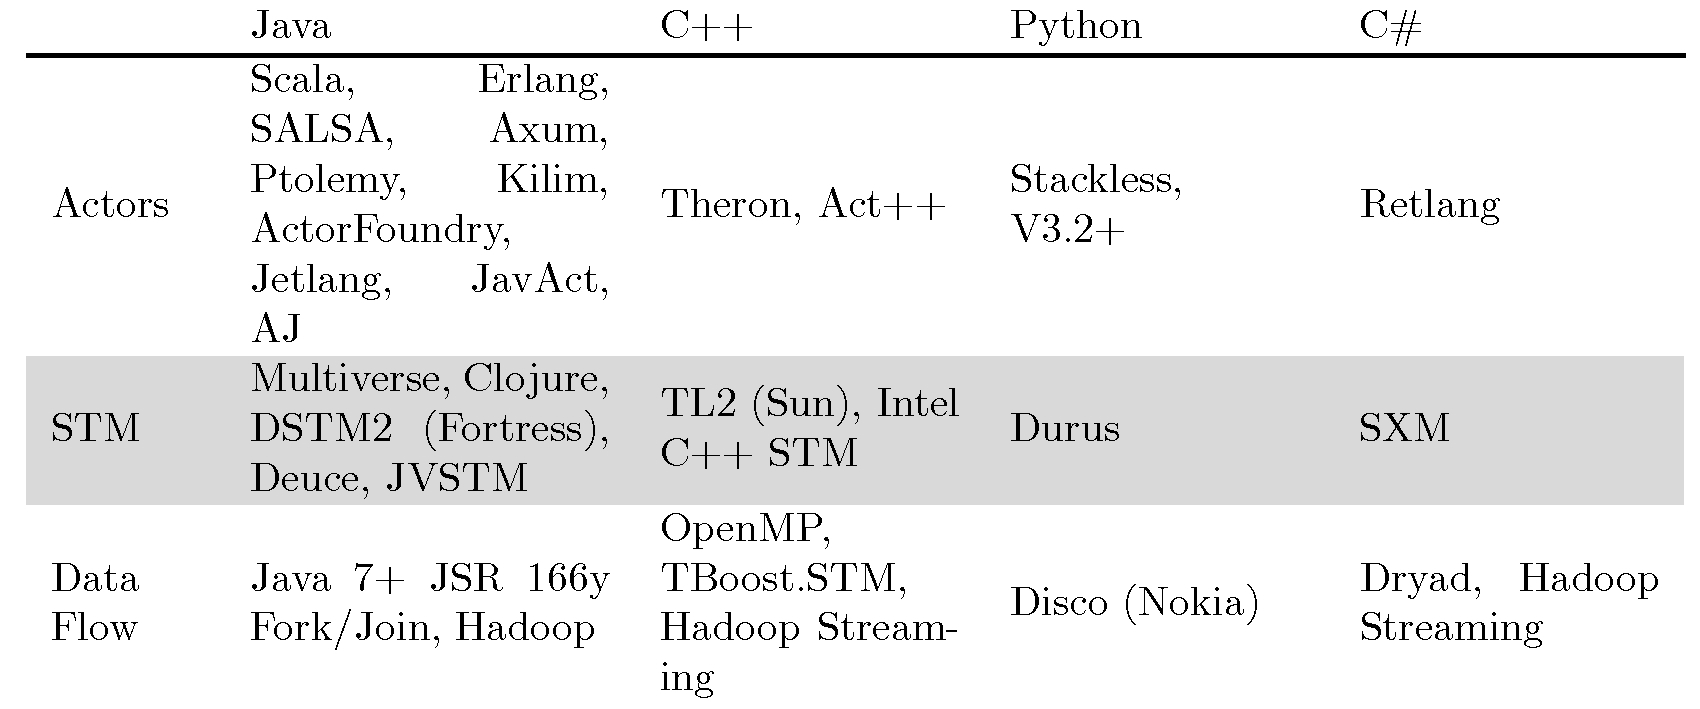
\includegraphics[scale=.85]{langs}
%\caption{Languages and libraries in different paradigms}
%\label{tbl:langs}
%\end{center}
%\end{table}

% SALSA \cite{salsa:agha} is an actor-based
%language for mobile and Internet computing that provides three significant
%mechanisms based on actor model: token-passing continuations, join
%continuations, and first-class continuations. 
%%
%Ptolemy \cite{ptolemy_ii:lee} is
%an actor-oriented open architecture and platform that is used to design, model
%and simulate embedded software. Their approach is hardware software co-design.
%It provides a platform framework along with a set of tools. 
%%
%Axum \cite{axum} is
%a language that builds upon the architecture of the Web and principles of
%isolation, actors, and message-passing to increase application safety,
%responsiveness, scalability, and developer productivity. 
%%
%Kilim \cite{kilim:Srinivasan_Mycroft} is a framework used to create robust and
%massively concurrent actor systems in Java. It uses a bytecode post-processor
%called Weaver \cite{kilim:Srinivasan_Mycroft}. Kilim takes advantage of code
%annotations on bytecode to provide the facility. 
%%
%ActorFoundry
%\cite{actor_frameworks_jvm:agha}] is a Java framework that brings the actor
%model implementation to the developer through the use of code annotations. It
%provides fair scheduling, actor mobility, and safe messaging out of the actor
%semantics. 
%%
%DPJ \cite{dpj} is a project aiming to provide
%deterministic-by-default semantics for an object-oriented, imperative parallel
%language, using primarily compile-time checking.

%
%Multiverse \cite{multiverse_homepage} is a Java based STM implementation that
%aims at seamless integration in the language and language independence in the
%form a framework. Clojure \cite{clojure:web,clojure_concurrent:web} is a dynamic
%programming language as a dialect of LISP that target Java Virtual Machine.
%Clojure provides concurrent programming constructs based on STM concepts. JVSTM
%\cite{jvstm}, another Java based STM library, introduces two core concepts as
%``transactions'' and ``versioned boxes''.
%%The goal is to allow
%% transaction programming at the programming language level, independent of an external
%%transaction manager.

%Java 7 \cite{java7} is supposed to provide language-level features for data flow
%programming as proposed in JSR 166y \cite{jsr166} including fork/join. The
%Apache Hadoop project \cite{hadoop} develops software for reliable, scalable,
%distributed computing proposing several frameworks among which is MapReduce
%\cite{hadoop_mapreduce} that is a framework for distributed processing of large
%data sets on computer clusters.
%
%Act++ \cite{actpp} is a class library for concurrent programming in C++ using
%actors model. Theron \cite{theron} is a lightweight, portable C++ class library
%for developing parallel applications. It implements a simple service-oriented
%model of concurrent processing based on Actor Model.
%
%Intel C++ STM Compiler \cite{intel_cpp_stm_v4} is a C++ platform that provides
%STM concepts of isolation and atomic executions in a C++ compiler. Transactional
%Locking II (TL2) \cite{tl2} is an STM algorithm based on a combination of
%commit-time locking and a novel global version-clock based validation technique.
%TBoost.STM \cite{tboost.stm} is another C++ library that provides STM
%implementation.
%
%The most prominent feature of Stackless Python \cite{stackless_python} is
%\textit{microthreads}, which avoid much of the overhead associated with usual
%Moreover, Python 3.2 \cite{python.3.2} introduces a library for future
%computation based on thread pooling. Durus \cite{durus} is a simple, yet mature,
%complete and fast, STM implementation for Python, allowing both STM inside a
%single process and STM in a server/multiple clients architecture. Disco
%\cite{disco} is a distributed computing framework based on the MapReduce
%paradigm.
%%operating system threads.
%%This avoids many of the overheads of threads, because
%%no mode switching between user mode and kernel mode needs to be done, and can
%%significantly reduce CPU load in some high-concurrency situations.
%
%Retlang \cite{retlang} is intended for use in message based concurrency similar
%to event based actors in Scala. The library does not provide remote messaging
%capabilities. It is designed specifically for high performance in-memory
%messaging.


%%%%%%%%%%%%%%%%%%%%%%%%%%%%%%%%%%%%%%%%%%%%%%%%%%%%%%%%%%%%%%%%%%%%%%%%%%%%%%%%%%%%%%%%%%%%%%%%%%%%

% Agha, in \cite{actors:agha}, introduces ``Actors'' as an inherently concurrent
% programming model. According to \cite{actor_frameworks_jvm:agha}, in the Actor
% model, systems comprise of concurrent and autonomous entities called
% \textit{actors} and \textit{messages}. Actors communicate by sending
% asynchronous messages to other actors for which they should be aware of the
% destination actor \textit{name} (mailbox).
% %Each actor in response to the
% %receiving messages can display different behavior as \cite{actors:agha}
% %proposes:
% %\begin{enumerate}
% %  \item Send a finite set of messages to other known actors;
% %  \item Create a a finite set of new actors; and
% %  \item Define how it will behave in relation to the next incoming messages
% %\end{enumerate}
% %In actor model, there is an extensive usage of ``pattern matching'' for messages
% %that are entrant to the mail box of an actor. This is also important in case of
% %an internal representation of actor. When a programmer is writing an actor, she
% %needs to specify the messages to which the actor will respond. 

% Actor model supporters also tend to take much advantage of ``pattern matching''
% and  ``functional programming'' concepts
% \cite{actors_highly:Correa,erlang:armstrong,salsa:agha,scala_actors:ordersky}.
% \cite{actor_frameworks_jvm:agha} provides a good comparison of the frameworks
% implemented for JVM platform. Moreover, \cite{wiki:actors:impl} provides some of
% the implementing languages and libraries.
% 
% Shavit and Touitou \cite{stm_shavit_touitou} introduce software transactional
% memory as a method for supporting transactional programming  of synchronized
% operations. They use STM to provide a general concurrent method for translating
% sequential object implementations to non-blocking ones. The most important
% property of STM is its \textit{non-blocking} nature as opposed to lock-based
% programming models. A \textsl{transaction} is finite sequence of local and
% shared memory machine instructions \cite{stm_shavit_touitou}. Transactions are
% \textit{isolated} and \textit{atomic}; the former means that each transactions
% runs as if others are suspended while it runs and the latter means that they are
% all-or-nothing operations \cite{stm_Adl-Tabatabai}. Thus, they give the
% programmer the illusion of a serial execution. \cite{wiki:stm:impl} provides
% some of the implementations of STM in different languages.
% 
% %Accordingly, \cite{stm_shavit_touitou} proposes that a software transactional
% %memory is \textit{shared object} that behaves like a memory that supports
% %multiple changes to its addresses by means of transactions. A transaction is a
% %thread of control that applies a finite sequence of primitive operations to
% %memory. This is why software transactional memory is believed to bring in the
% %concept of database transactions on data into object-oriented paradigm. In this
% %model, each object provides a set of \textit{primitive operations} only through
% %which the underlying object (shared memory) can be manipulated. 
% %\cite{stm_shavit_touitou} introduces \textit{wait-free}, \textit{non-blocking},
% %and \textit{swap-tolerant} transactions as types of STM.
% 
% Data flow programming \cite{dataflow_prog:wiki}, that can be considered a branch
% of flow-based programming \cite{flow_prog:wiki}, focuses on facilitating
% parallel computation through division, conquering and merging of a program based
% on the data on which it processes. Based on data flow programming, in
% \cite{mapreduce:dean_ghemawat}, they propose MapReduce that is basically based
% on one \textit{map} and one \textit{reduce} function. It is originally proposed
% and extensively used at Google. The programmer writes two function. ``Map''
% takes an input pair and produces a set of intermediate \textsl{key/value} pairs.
% When the computation is done, the library groups together all intermediate
% values associated with the same intermediate key and passes them to reduce
% function. ``Reduce'' function accepts an intermediate key and all the grouped
% associated values and it is supposed to merge the values to possibly form a
% smaller set of values. For instance, in \cite{mapreduce_ml:cheng}, they use
% MapReduce in Machine Learning purposes.
% 
% Philippsen in \cite{survey_mcp:philippsen} categorizes the problems of
% concurrent object-oriented languages (COOL) as \textit{parallel performance},
% \textit{broken encapsulation}, \textit{inheritance anomalies}, and
% \textit{expressive coordination constraints}. He provides a complete comparison
% of the languages based on the problems; yet the languages used are as of to the
% end of 2000. A more complete of the different concurrent languages can be found
% at \cite{concurrent_lang_list:wiki}.
% %Table \ref{tbl:langs} provides a brief overview of the some of the
% %current languages and libraries. 
% 
% %\begin{table}[t]
% %\begin{center} 
% %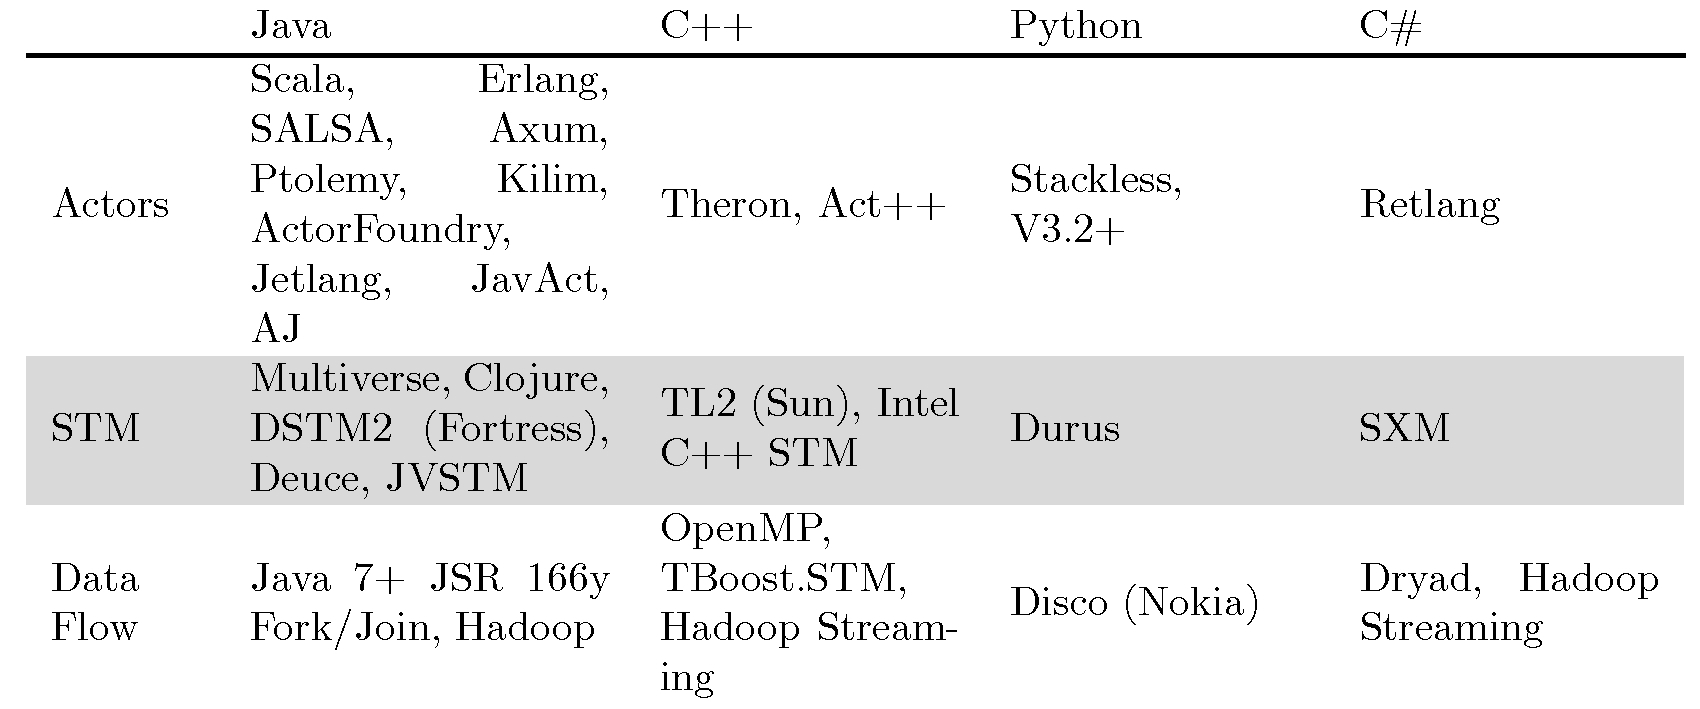
\includegraphics[scale=.85]{langs}
% %\caption{Languages and libraries in different paradigms}
% %\label{tbl:langs}
% %\end{center}
% %\end{table}
% 
% Erlang \cite{erlang:armstrong} is a dynamically typed functional language that
% was developed at Ericsson Computer Science Laboratory with telecommunication
% purposes \cite{actors_highly:Correa}. SALSA \cite{salsa:agha} is an actor-based
% language for mobile and Internet computing that provides three significant
% mechanisms based on actor model: token-passing continuations, join
% continuations, and first-class continuations. Ptolemy \cite{ptolemy_ii:lee} is
% an actor-oriented open architecture and platform that is used to design, model
% and simulate embedded software. Their approach is hardware software co-design.
% It provides a platform framework along with a set of tools. Axum \cite{axum} is
% a language that builds upon the architecture of the Web and principles of
% isolation, actors, and message-passing to increase application safety,
% responsiveness, scalability, and developer productivity. Scala is a hybrid
% object-oriented and functional programming language inspired by Java in which a
% famous Actors library exists that mimics the Erlang implementation. The most
% important concept introduced in \cite{scala_actors:ordersky,coord:ordersky} is
% that Scala Actors unifies \textit{thread-based} and \textit{event-based}
% programming model to fill the gap for concurrency programming.
% %In this model, an
% %actor is a thread that can also \textit{react} to events that come in from other
% %actors; i.e. it provides both \texttt{receive} and \texttt{react} features.
% %\texttt{react} is a complement to \texttt{receive} that is proposed in the
% %original actor model. 
% Kilim \cite{kilim:Srinivasan_Mycroft} is a framework used to create robust and
% massively concurrent actor systems in Java. It uses a bytecode post-processor
% called Weaver \cite{kilim:Srinivasan_Mycroft}. Kilim takes advantage of code
% annotations on bytecode to provide the facility. ActorFoundry
% \cite{actor_frameworks_jvm:agha}] is a Java framework that brings the actor
% model implementation to the developer through the use of code annotations. It
% provides fair scheduling, actor mobility, and safe messaging out of the actor
% semantics. DPJ \cite{dpj} is a project aiming to provide
% deterministic-by-default semantics for an object-oriented, imperative parallel
% language, using primarily compile-time checking.
% %“Deterministic” means that the
% %program produces the same visible output for a given input, in all executions. 
% %“By default” means that deterministic behavior is guaranteed unless the
% %programmer explicitly requests nondeterminism.
% 
% Multiverse \cite{multiverse_homepage} is a Java based STM implementation that
% aims at seamless integration in the language and language independence in the
% form a framework. Clojure \cite{clojure:web,clojure_concurrent:web} is a dynamic
% programming language as a dialect of LISP that target Java Virtual Machine.
% Clojure provides concurrent programming constructs based on STM concepts. JVSTM
% \cite{jvstm}, another Java based STM library, introduces two core concepts as
% ``transactions'' and ``versioned boxes''.
% %The goal is to allow
% % transaction programming at the programming language level, independent of an external
% %transaction manager.
% 
% Java 7 \cite{java7} is supposed to provide language-level features for data flow
% programming as proposed in JSR 166y \cite{jsr166} including fork/join. The
% Apache Hadoop project \cite{hadoop} develops software for reliable, scalable,
% distributed computing proposing several frameworks among which is MapReduce
% \cite{hadoop_mapreduce} that is a framework for distributed processing of large
% data sets on computer clusters.
% 
% Act++ \cite{actpp} is a class library for concurrent programming in C++ using
% actors model. Theron \cite{theron} is a lightweight, portable C++ class library
% for developing parallel applications. It implements a simple service-oriented
% model of concurrent processing based on Actor Model.
% 
% Intel C++ STM Compiler \cite{intel_cpp_stm_v4} is a C++ platform that provides
% STM concepts of isolation and atomic executions in a C++ compiler. Transactional
% Locking II (TL2) \cite{tl2} is an STM algorithm based on a combination of
% commit-time locking and a novel global version-clock based validation technique.
% TBoost.STM \cite{tboost.stm} is another C++ library that provides STM
% implementation.
% 
% The most prominent feature of Stackless Python \cite{stackless_python} is
% \textit{microthreads}, which avoid much of the overhead associated with usual
% Moreover, Python 3.2 \cite{python.3.2} introduces a library for future
% computation based on thread pooling. Durus \cite{durus} is a simple, yet mature,
% complete and fast, STM implementation for Python, allowing both STM inside a
% single process and STM in a server/multiple clients architecture. Disco
% \cite{disco} is a distributed computing framework based on the MapReduce
% paradigm.
% %operating system threads. 
% %This avoids many of the overheads of threads, because
% %no mode switching between user mode and kernel mode needs to be done, and can
% %significantly reduce CPU load in some high-concurrency situations. 
% 
% Retlang \cite{retlang} is intended for use in message based concurrency similar
% to event based actors in Scala. The library does not provide remote messaging
% capabilities. It is designed specifically for high performance in-memory
% messaging.
% 
% %\subsection{Discussion}
% %
% %Many of the well-known languages provide language constructs enabling the
% %programmer to take advantage of multicore technology. The language features
% %include concepts such as conditions, atomic data structures, and locks among
% %others. They all provide the required fundamentals to build more complex data
% %structures and programs that need to take advantage of concurrent objects on
% %multicore. Though, they also introduce new challenges in accordance: 
% %
% %\begin{description}
% %  \item[Level of abstraction.] Although the language constructs for multicore
% %  are based on a high-level paradigm such as object orientation, they seem to be
% %  still in lower levels of abstraction expected for multicore. In other words,
% %  the current feature set provide sound primitives for programming multicore
% %  yet to grow mature to higher level of abstraction for simpler use.
% %  \item[Composability.] Another interesting challenge of using language
% %  primitives to construct concurrent objects is how to use them in use cases of
% %  composition to build larger programs. Composing pieces of code to build
% %  larger code often bring in the problem of complexity. The complexity in this
% %  area rises up in the form of synchronization issues required to be resolved by
% %  the programming technique adopted by the programmer. In this line, Aka
% %  (REF???) is an interesting attempt to create a hybrid solution to alleviate the
% %  challenges.
% %  \item[Level of expertise.] Generally speaking, it is the responsibility of the
% %  programmer to come up with a correct and efficient design how to use the
% %  language fundamental features to build a more complicated program. In essence,
% %  this capability depends on the level of experience, skill, and knowledge
% %  of programming concepts. It is more desirable to propose and provide
% %  higher-level yet simpler programming language constructs so that the
% %  programmer can easily take advantage with little concern on the level of expertise
% %  required to use them.
% %\end{description}
% %
% %In another line of research efforts, libraries have been developed to provide a
% %solution on top of a language for concurrent objects on multicore. Development
% %of libraries give rise to concerns:
% %\begin{description}
% %  \item[Side Effects.] Usually the compiler of the language does not know
% %  about the semantics of the added library meaning that it may bring side
% %  effects to the correctness of the executing code \cite{survey_mcp:philippsen}.
% %  \item[Compiler Optimizations.] In another insight into library development,
% %  the compiler optimization process is missed out for the extra code since the
% %  compiler is not accordingly instrumented to act upon the new code for the
% %  added library \cite{survey_mcp:philippsen}. Optimizations may become important
% %  in case of heavy processing needs or limitations of resources.
% %  \item[Coverage.] Another interesting point in library development is that
% %  libraries are \textit{usually} developed with specific directions or concerns.
% %  This means that they do not consider all the concerns in concurrent objects
% %  concepts for the purpose of simplicity or prototyping 
% %  \cite{survey_mcp:philippsen}.
% %\end{description}
% 
% 
% 
